\chapter{Distributed computing}

As mentioned, The Wind Power Supervisor (WPS) and the Park Pilot does not scale well with the number of turbines, which forces Siemens to set the regulation cycle time after worst case scenarios (see \cref{sec:SiemensCase} for details). Today this cycle time is set to 150 ms and Siemens wants the time reduced to 10 ms. This is a major performance improvement and as such not a strict demand from the Siemens case, meaning any reduction in the 150 ms cycle time will be accepted. The goal for the decentralized solution to the Siemens case is therefore to reduce the regulation cycle time as much as possible.

Looking at the park regulation algorithm \cref{sec:SiemensCase}, the reason for it being slow is primarily the communication overhead involved, when requesting set points from every turbine and sending new set points to every turbine, and that this communication overhead increases with the number of turbines involved with the regulation. So to reduce the regulation cycle time, this communication overhead needs to be reduced, by letting each turbine perform park regulations and calculate their own set points. 

Removing the communication overhead from the regulation algorithm involves detaching sharing of data from the algorithm. In order to do this

For the Park Pilot to be able to compute a park regulation, the Park Pilot needs information about every turbine in the farm. In the same way, when decentralizing the Park Pilot, if a turbine is to compute park regulations, the turbine needs information about every other turbine. This means the windmill farm needs a global shared state, where information about every turbine in the farm is available to every turbine performing park regulations. 

%This is a major performance improvement and for that reason, performing the regulation sequence using a distributed database only is not enough, since reading/writing to the disk takes valuable milliseconds. Therefore regulation information needs to be kept in memory in order to keep regulation cycle time as low as possible. 

This chapter describes and discusses different distributed computing paradigms as a way of making a global state for the turbines to compute park regulations themselves. The goal is to find the paradigm best suited for the Siemens case. Furthermore, the chapter describes relevant technologies within the chosen paradigm and discusses which technology that is the best for the Siemens case.

The chapter uses the following definition by Andrews~\cite{andrews2000foundations} for distributed computing: \textit{In distributed computing, each node or process has its own local memory and communication happens via message passing.}



%Furthermore, when decentralizing the Wind Power Supervisor onto the turbines, the turbines obviously needs to be able to handle external data aggregation . For the heavy tasks, in terms of CPU power, distributed computing becomes relevant as a way of improving performance by combining the CPU power residing inside the turbines to compute a common task.

%
%In distributed computing, each node or process has its own local memory and communication happens via message passing~\cite{andrews2000foundations}. This means distributed computing is a way of having a global system state and keep relevant information, with regards to the global state, in memory, and thereby avoid read/write operations to the disk. 



\section{Message passing}

Message passing is a low-level communication paradigm, where processors communicate by sending messages via bidirectional channels. It is a highly used paradigm and other communication paradigms are usually implemented on top of an underlying message-passing system.  

With message passing being a low-level communication paradigm, the communication overhead is low compared to paradigms build on top of it. It is entirely up to the application developer to handle communication. This will in many cases result in better execution time, which is the most compelling argument for choosing message passing as communication paradigm. The problem with it being up to the developer, is that the developer needs to deal with configurations setup, such as sockets and marshaling, exception handling and who and when to communicate with when developing the application. This makes it hard to develop using message passing, especially when dealing with more complex applications~\cite{lu1995message}. 


\section{Distributed shared memory}

Shared memory is an attractive paradigm for designing parallel and distributed systems. Applications can use shared memory as a tool for the entire system to share a common state. However for loose coupled distributed systems, no physically shared memory is available to support such a model. Distributed shared memory (DSM) is a way of providing physically distributed memory machines a shared memory abstraction, illustrated on \cref{fig:distributedSharedMemory}.

\begin{figure}
	\centering
	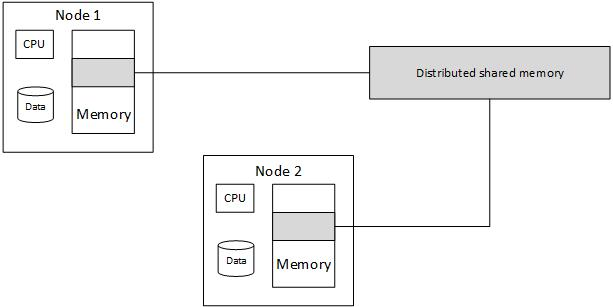
\includegraphics[width=0.8\textwidth,natwidth=610,natheight=642]{DistributedSharedMemory.jpg} 
	\captionsetup{format=plain,font=footnotesize,labelfont={bf,defaultCapFont},labelsep=quad,singlelinecheck=no}
	\caption[Distributed Computing System with 2 nodes]{
		\label{fig:distributedSharedMemory} 
		\footnotesize{%
			A distributed shared memory system with 2 nodes.
		}
	}
\end{figure}

The primary advantage of DSM is the shared memory abstraction provided. This gives the illusion of physically shared memory and allows developers to use the shared-memory paradigm, without having to think about communication mechanisms. For this reason the DSM paradigm is fully decoupled in space, since producers and consumers of data remain anonymous to each other, and in time, since the producers needs no knowledge of future use of the data. Synchronization decoupling is achieved by some implementations of DSM, where each node keeps local copies of the shared data~\cite{guedes1993distributed}.

A downside to the DSM abstraction is that it introduces overhead to the system, since the DSM abstraction has limited knowledge of the application flow, compared to communication via message passing~\cite{lu1995message}. 

 

%DSM pass by reference

%In distribted system there might be scenarios in which a task waits for a service at the queue of one resource, while at the same time another resource which is capable of serving the task is idle. The purpose of a load balancing algorithm is to prevent these scenarios as much as possible.

%three phases.
%Information collection: Gathers info of workload
%decision making: Calc optimal data dist.
%data migration: Transfer excess amount of workload from on overloaded processor to another underloaded processor

%Centralized: Size of grid increases, keppeing all the inforation about the state of all the resources is a bottlebeck. Scalability becomes an issue. Page 281. 

%The benifits of this technique stems from Load Balancing
%State Broadcast Algorithm (SBA). Page 282

%Basic assumptions Page 289.

%Scalability and makespan (Y). Page 298, conclusion.


\section{Publish/subscribe}

Publish/subscribe is a messaging pattern where communication is interest based instead of address based. Messages are characterized into classes and sent by publishers, without knowledge of how many subscribers there may be. Nodes can then subscribe to one or more classes of interest, without knowledge of how many publishers there are, providing a more decoupled, scalable and flexible interaction model.

\begin{figure}
	\centering
	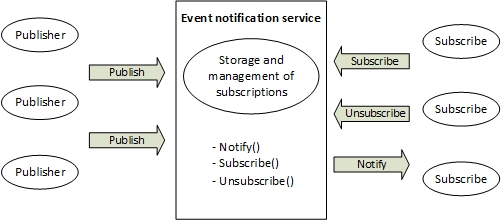
\includegraphics[width=0.9\textwidth,natwidth=610,natheight=642]{PublishSubscribe.jpg} 
	\captionsetup{format=plain,font=footnotesize,labelfont={bf,defaultCapFont},labelsep=quad,singlelinecheck=no}
	\caption[Distributed Computing System with 2 nodes]{
		\label{fig:publishSubscribe} 
		\footnotesize{%
			A simple publish/subscribe system.
		}
	}
\end{figure}

The publish/subscribe paradigm is event driven and corresponds to the observer design pattern, where subscribers are registered via keywords instead of registering their interest directly with the publishers. The paradigm relies on an event notification service providing storage and management for subscriptions and efficient delivery of events, as illustrated on \cref{fig:publishSubscribe}. The subscribers are notified subsequently of any event, generated by a publisher, matching the registered interest. The strength of this event-based communication is the full decoupling in time, space and synchronization between publishers and subscribers~\cite{eugster2003many}.

%Quality of service??

% DSM is only space and time decoupled but not sync, because consumers pull from shared space in a synchronous style


\section{Remote procedure call}

Remote procedure call (RPC) is a communications paradigm built for client/server architecture~\cite{Microsoft2003RPC}, which makes remote interactions appear the same way as local interactions. The goal is to make the process of executing code on a remote machine as simple as calling a local function~\cite{dusseau2014intro} by factoring out common tasks, such as security, synchronization, and data flow handling. This explains the paradigms popularity in distributed computing. However distribution cannot be made completely transparent to the application, because it gives rise to further types of potential failures, like communication failures, that have to be dealt with explicitly~\cite{coulouris2005distributed}. 

The idea of RPC is quite simple. When a remote procedure is invoked, the calling environment is suspended, the parameters are passed across the network to the environment where the procedure is to execute and the desired procedure is executed at that location. When execution is finished, return values are sent back to the calling environment, where execution resumes \cite{birrell1984implementing}.

A shortcoming of RPC is the strong coupling in time, space and synchronization. Although solutions have been presented to remove the synchronization coupling by future remote invocation. Remote method invocation is a paradigm where RPC as been applied to object-oriented contexts~\cite{eugster2003many}.

%Not appropriate for broadcasting

%Strong time coupled 
%sync coupled from the consumer side (waits for the return of the call, calling environment is suspended). Can be changed so sender does not expect reply (weak reliablity, no success or failure). Or return handle for sender to later request return value when needed (future remote invocation)

%Space coupling (remote reference to object)


%\section{Notification}
%
%The notification paradigm corresponds to the observer design pattern. It works by having subscribers register their interest directly with the publishers, which manages subscriptions and send events. It is usually implemented using two asynchronous invocations, in order to enforce synchronization decoupling: the first is sent by the client to the server, containing invocation arguments and a callback reference to the client, and the second is sent by the server to the client to return one or more replies. However publishers and subscribers remain coupled in time and space. Furthermore the communication management is left to the publisher. This can become a problem as the system grows in size \cite{eugster2003many}.

%Publish/Subscribe where subscribers register their interest directly with publishers, which manages subscriptions and send events.

%event driven

%\section{Message queuing}
%Message queuing is a message-centric approach that usually integrate some form of publish/subscribe transaction. It works by having producers append messages to a global FIFO or priority queue asynchronously and consumers dequeue them synchronously from that same queue, where messages can only be consumed by one consumer. At an interaction level message queues recall much of DSM, where producers feed messages to some global memory space. Similarly to DSM, producers and consumers are decoupled in both space and time, where synchronous decoupling is only present for the producers \cite{eugster2003many}.

%Global FIFO kø. Til hvis man er ligeglad med, hvem der tager opgaven??


%\begin{table}
%	\begin{tabular}{l >{\centering}m{5cm} c}
%		\hline
%		\hline
%		\textbf{Abstraction} & \textbf{Space} & \textbf{Time} & \textbf{Flow} \\
%		\hline
%		\hline
%		Message Passing & \checkmark & \checkmark \\
%		\hline
%		RPC/RMI & \checkmark & \checkmark \\
%		\hlines
%		Async. RPC/RMI & \checkmark & \checkmark \\
%		\hline
%		Future RPC/RMI & \checkmark & \checkmark \\
%		\hline
%		Notifications & \text{x}& \text{x} & \checkmark \\
%		\hline
%		DSM & \checkmark & \checkmark & P(\checkmark) \\
%		\hline
%		Message Queuing (PULL) & \checkmark & \checkmark & \text{P(} \checkmark \text{)} \\
%		\hline
%		Public/Subscribe & \checkmark & \checkmark & \checkmark \\
%		\hline
%		\hline
%	\end{tabular}
%	
%	\caption[MongoDB VoltDB]{
%		\label{tab:mongovolt}
%		\footnotesize{%
%			Comparison of MongoDB and VoltDB.
%		} 
%	}
%\end{table}

\section{Comparison with regards to the Siemens case}
Looking at the Siemens case (\cref{sec:SiemensCase}) the new distributed system must act as a single unit, be able to perform park regulations and scale easily with the number of turbines. Furthermore Siemens wish to remove single point of failures. With this in mind, the remote procedure call paradigm is not an option because it is tight coupled and build for a client/server architecture, which is exactly what Siemens is trying to avoid. One could imaging using a partial client/server architecture, with a communication hierarchy, however this would introduce some communication overhead~\cite{Yu1997JavaDSM} and single point of failures to the system.

As mentioned, to perform the park regulation sequence, the windmill farm needs a global shared state, where information about every turbine available to every turbine performing park regulations. Therefore, if the decentralized version of the Siemens case were to be implemented using raw message passing, it would result in building some kind of DSM and/or publish/subscribe abstraction, with roughly the same communication overhead. To save the trouble of developing this abstraction, we conclude that message passing is not an option as communication paradigm.

This leaves DSM and publish/subscribe as remaining paradigms, where one could imagine the Siemens case being implemented using either of the two. The abstraction of shared memory provided by DSM is attractive when looking looking at the Siemens case. As a system developer, being able to think of the global shared state as local memory is to prefer over event handling. Therefore DSM is chosen over publish/subscribe since publish/subscribe introduces event handling to the system.

% The abstraction provided by DSM is attractive when looking looking at the Siemens case. As a system developer, being able to think of the global shared state as local memory is to prefer over thinking about communication semantics. However before before choosing, it is relevant to look at the cost of the DSM abstraction.

%\subsection{Message passing or DSM?}
%
%The abstraction provided by DSM is attractive when looking looking at the Siemens case. As a system developer, being able to think of the global shared state as local memory is to prefer over thinking about communication semantics. However before before choosing, it is relevant to look at the cost of the DSM abstraction.

%Comparing DSM with message passing in terms of processing time and network communication time is not entirely fair since DSM is an abstraction built using message passing. Therefore, Honghui~\cite{lu1995message} argues that it is hard for DSM to outperform message passing, in terms of application execution time, given the larger software-overhead. Honghui has studied and compared a DSM system with message passing system, with the goal to assess the differences in application development time and program execution time between DSM and message passing, and determine the causes of the lower program execution time of DSM systems. He ported 12 different parallel program scenarios to a DSM system called TreadMarks and a message passing system called PVM. For 5 of the scenarios, TreadMarks performed within 10\% of PVM. For 6 of the programs the difference were between 10\% - 30\%. For the last scenario, PVM performed twice as well as TreadMarks. 
%
%%He ported 12 different parallel program scenarios to a DSM system called TreadMarks and a message passing system called PVM and compared the two technologies with regards to programmability and performance. He argues that given DSM is an abstraction built on top of message passing, DSM cannot achieve better performance than message passing, given the larger software-overhead. Therefore the goal is to achieve the same performance as message passing using DSM. For 5 of the scenarios, TreadMarks performed within 10\% of PVM. For 6 of the programs the difference were between 10\% - 30\%. For the last scenario, PVM performed twice as well as TreadMarks. 
%
%Honghui argues that the program execution time is dependent of the logical flow of the program scenario. More messages and more data are sent in TreadMarks, explaining the performance differences. He gives the following reasons for the extra communication in TreadMarks:
%
%\begin{itemize}
%	\item Separation of synchronization and data transfer in TreadMarks. 
%	\item Extra messages to request updates for data in the invalidate protocol used in TreadMarks.
%	\item False sharing.
%	\item Diff accumulation for migratory data in TreadMarks.
%\end{itemize} 
%
%%1) Seperation of synchronization
%% Lazy release consistency: Against data races (which may result uin wrong results). Only the next processor that acquires the lock can access x --> only that processor is informormed of the change to x --> reduce message traffic. Ex: Barriers - No processor overites values before all processors have read the value computed in the previous interation.
%
%%2) Extra messages to request updates for data in the invalidate protocol used in TreadMarks
%% Memory page change communicatin. Modified pages are inviladated after an acquire. Later access causes access miss, which in turn causes installation of an up-to-date copy of the page.
%
%%3) False sharing
%% To objects er allokerede i samme memory page og de skrives til samtidig --> force update af page --> overhead
%
%%4) diff accumulation for migratory data in TreadMarks
%% Multiple-writer protocol to allow wrinting on same page at the same time. Uses a diff algorithm to reduce false sharing effects.
%
%Honghui concludes that the performance of a well optimized DSM system is comparable to that of a message passing system. Furthermore, development of systems with complex communication patterns takes a lot less effort using the DSM paradigm.
%
%In contrast to Honghui, Stumm and Zhou~\cite{stumm1990algorithms} argues that applications using DSM can in fact outperform their message passing counterparts, in a few cases. They argue, that this is possible for the following reasons:
%
%\begin{itemize}
% 	\item DSM algorithms typically move data on demand as they are being accessed, which spreads communication load over a longer period of time, allowing for a greater degree of concurrency. If for example a node uses the shared memory more than others, the node does not need to communicate for every write operation made to the shared memory.
% 	\item For DSM algorithms that sends data in large blocks, communication overhead is reduced. 
%\end{itemize} 
%
%Looking at the Siemens case the two major factors for the communication paradigm choice are scalability and availability.
% With that in mind, BLABLA is not an option because of .. 
%
%Message queuing and RMI offers feature which  



\section{State of the art DSM}

The regulation algorithm is a recursive algorithm, which performs calculations of new turbine set points using the following parameters:

\begin{itemize}
	\item Current state of every turbine in the farm.
	\item Max capacity of each turbine.
	\item Historic data from previous calculations.
\end{itemize} 



In order to remove the communication overhead from the regulation cycle time, information sharing through the chosen paradigm, DSM, needs to to be detached from the regulation cycle. 

Looking at the global shared state 

 Removing communication overhead from the park regulation cycle involves the following

DSM is a paradigm well implemented through by many different frameworks, with their own individual and unique implementation.


Therefore, to determine which technology that is best suited for the Siemens case, the technologies will be compared on the following set of parameters: 

%standalone: Type?
%Distributed shared memory support
%Distributed shared chache support
%Distributed memeory support
%Performance
%Client/server?
%Framework architecture. distributed shared memeory, client/server or not  
%cost

With DSM chosen as the communication paradigm, this chapter describes, evaluates and discusses different DSM technologies in order to find the technology best suited for Siemens.

%Standalone, avoid overhead


\section{In memory databases}
%Client/server architecture

\section{In-memory data grids}
%Distributed memory. Only shared for replica reasons

\subsection{Oracle Coherence}
%dist. memory --> distributed chache
%java, .net, c++
%http://www.oracle.com/technetwork/middleware/coherence/distributed-caching-100021.html


\subsection{VMware Gemfire}
%Contact sales
%Not open source

\subsection{Gigaspaces XAP}
%Share nothing architecture

\subsection{ScaleOut Software}
%Java, .NET, C/C++ 
%cash
%Share nothing architecture
%http://www.scaleoutsoftware.com/downloads-resources/downloads/

\subsection{NCache}
%expensive
%http://www.alachisoft.com/ncache/index.html

\subsection{Hazelcast}
%java
%opensource
%http://hazelcast.com/products/hazelcast/

\section{Distributed shared cache}


\subsection{jBoss Cache}
%Java 5.0 and 6
%forældet


\subsection{DSM in .NET}
%IP multicast

%casusally consistent: Writes that are potentially causally related must be seen by all processes in the same order. Concurrent writes may be seen in a different order on different machines.

\subsection{AppFabric}
%Runs on IIS


\subsection{DDS}


\section{Conclusion}

%Ens
%Valg med vægt på arkitektur og development tid. 
%RMI fravalg